\documentclass[17pt]{extarticle}
\usepackage{amsmath}
\usepackage{tikz}
\usepackage[top=0.2in,left=0.9in]{geometry} %This geometry is page layout


\begin{document}
\begin{flushleft}
Geometry Shapes :
\end{flushleft}


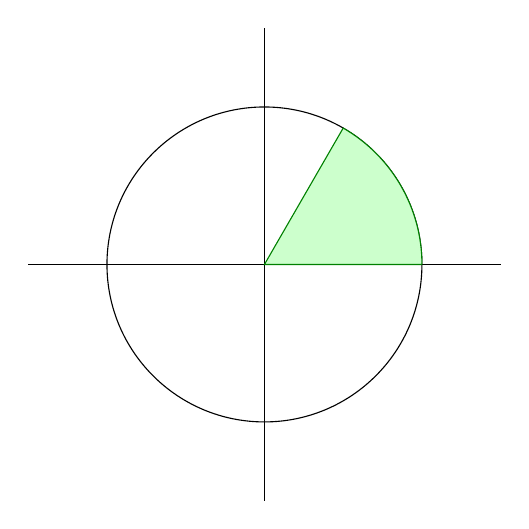
\begin{tikzpicture}
\draw (0,0) circle(2);
\draw (-3,0) -- (3,0);
\draw (0,-3) -- (0,3);

%Green Fill Arc
\filldraw[fill=green!20,draw=green!50!black] (0,0) -- (2,0) arc (0:60:2) -- cycle;
 \end{tikzpicture}
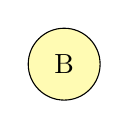
\begin{tikzpicture}
\node[draw, circle, fill=yellow!30, inner sep=2mm] (a) {B};
\end{tikzpicture}
\quad\quad

\begin{tikzpicture}
\shade (0,0) rectangle (2,1)
(3,0.5) circle (.5cm); 
\end{tikzpicture}

\quad\quad


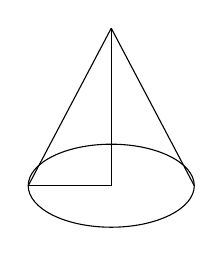
\begin{tikzpicture}
\draw (0,0) ellipse (30pt and 15pt);
\draw (0,0) -- (0,2);
\draw (0,0) -- (-30pt,0);
\draw  (-30pt,0) -- (0,2);
\draw  (30pt,0) -- (0,2);
\end{tikzpicture}



\end{document}


